\documentclass[tikz, border=10pt]{standalone}
\usepackage{tikz}
\usetikzlibrary{automata, positioning, arrows.meta}

\begin{document}

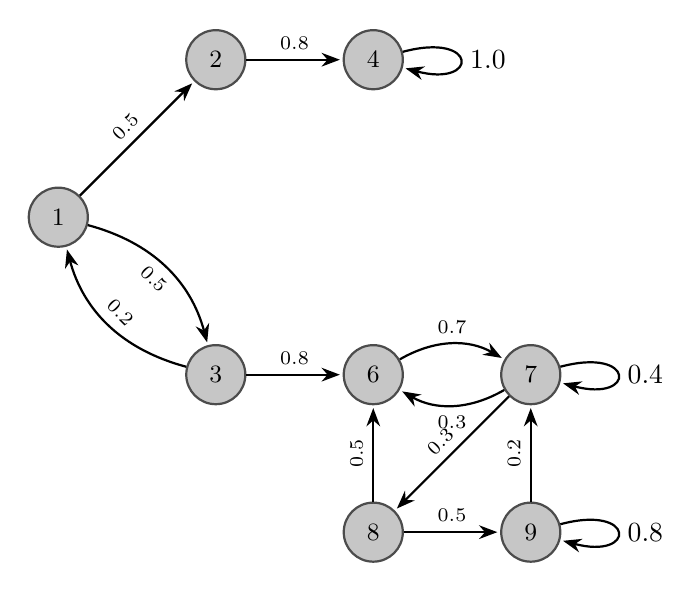
\begin{tikzpicture}[
    >=Stealth,
    shorten >=1pt,
    node distance=2cm,
    on grid,
    auto,
    state/.style={
        circle,
        draw=black!70,
        fill=darkgray!30,
        thick,
        minimum size=0.75cm,
        font=\small
    },
    prob/.style={
        font=\scriptsize,
        sloped,
        midway,
        above
    }, 
    scale=2
]

    % === États ===
    \node[state] (1) {$1$}; 
    \node[state, right of=1, above of=1] (2) {$2$};
    \node[state, right of=1, below of=1] (3) {$3$}; 
    \node[state, right of=2] (4) {$4$}; 
    \node[state, right of=3] (6) {$6$}; 
    \node[state, right of=6] (7) {$7$}; 
    \node[state, below of=6] (8) {$8$}; 
    \node[state, below of=7] (9) {$9$}; 

    % === Transitions avec probabilités ===
    \path[->, thick]
        (1) edge[above] node[prob] {$0.5$} (2)
        (2) edge[above] node[prob] {$0.8$} (4)
        (4) edge[loop right] node[right] {$1.0$} (4)
        (1) edge[bend left] node[prob, below] {$0.5$} (3)
        (3) edge[bend left] node[prob, above] {$0.2$} (1)
        (3) edge[above] node[prob] {$0.8$} (6)
        (6) edge[bend left] node[prob, above] {$0.7$} (7) 
        (7) edge[bend left] node[prob, below] {$0.3$} (6)
        (7) edge[loop right] node[right] {$0.4$} (7)
        (7) edge[right] node[prob] {$0.3$} (8)
        (9) edge[left] node[prob] {$0.2$} (7)
        (9) edge[loop right] node[right] {$0.8$} (9)
        (8) edge[below] node[prob] {$0.5$} (9)
        (8) edge[above] node[prob] {$0.5$} (6);

\end{tikzpicture}

\end{document}
